% Line Atlas chapter draft.
% Suggested dependencies: amsmath, amssymb, siunitx, booktabs, tabularx,
% tikz, pgfplots, xcolor, hyperref.

\chapter{The Multiphase Interstellar Medium, PDRs, and Molecular Gas}
\label{chap:ism-pdr-molecular}
\chaptermark{The Multiphase Interstellar Medium}

The interstellar medium (ISM) is a coupled system of gas, dust, magnetic fields,
cosmic rays, and radiation.  Its named ``phases'' are useful landmarks in density and
temperature, not sealed reservoirs.  Material moves among them through cooling,
heating, compression, rarefaction, ionization, recombination, molecule formation,
feedback, and galactic dynamics.  Spectral lines reveal this circulation because each
transition selects a different combination of abundance, excitation, optical depth,
and background.

The discussion here follows the physical framework developed in
\citet{Spitzer1978}, \citet{McKeeOstriker1977}, \citet{Draine2011}, and
\citet{Tielens2005}, with phase and small-scale qualifications discussed by
\citet{Cox2005} and \citet{StanimirovicZweibel2018}.  Photodissociation-region physics
is reviewed by \citet{HollenbachTielens1999}, and molecular conversion factors by
\citet{BolattoWolfireLeroy2013}.

\section{A phase is an equilibrium branch, not merely a temperature bin}

For an ideal gas with total particle density $n_{\rm tot}$,
\begin{equation}
 P_{\rm th}=n_{\rm tot}kT.
 \label{eq:thermal-pressure}
\end{equation}
Observers often quote $P_{\rm th}/k$ in units of
$\mathrm{K\,cm^{-3}}$.  Thermal pressure is only one part of the momentum budget:
\begin{equation}
 P_{\rm tot}=P_{\rm th}+P_{\rm turb}+P_B+P_{\rm cr}+P_{\rm rad},
 \qquad P_B=\frac{B^2}{8\pi}.
 \label{eq:total-ism-pressure}
\end{equation}
These terms need not be locally isotropic or in equipartition.  Magnetic tension, for
example, is not captured by treating $P_B$ as an ordinary scalar pressure.

The thermal energy equation can be written schematically as
\begin{equation}
 \frac{3}{2}n_{\rm tot}k\frac{\mathrm{d}T}{\mathrm{d}t}
 =\Gamma-n_en_{\rm H}\Lambda(T,\boldsymbol{x})
 -P_{\rm th}\boldsymbol{\nabla}\!\cdot\boldsymbol{v}
 +\boldsymbol{\nabla}\!\cdot(\kappa\boldsymbol{\nabla}T),
 \label{eq:thermal-energy-ism}
\end{equation}
where $\Gamma$ includes heating per volume, $\Lambda$ summarizes radiative cooling,
and the final terms represent compression or expansion and conduction.  In diffuse
neutral gas, photoelectrons ejected from small grains and polycyclic aromatic
hydrocarbons often provide important heating.  Cosmic-ray ionization, X-rays,
turbulent dissipation, and chemical heating can dominate in shielded or extreme
environments.  Cooling proceeds through species and transitions whose importance
changes with temperature, ionization, density, metallicity, and optical depth.

Thermal equilibrium satisfies $\Gamma=n_en_{\rm H}\Lambda$.  If heating scales
roughly as $n$ while cooling scales roughly as $n^2$, the equilibrium curve in
pressure-density space can have two stable branches separated by an unstable branch.
This motivates cold and warm neutral media that coexist over a range of pressure
\citep{WolfireEtAl2003}.  Turbulence continuously drives gas away from exact
equilibrium, so observed distributions are broad rather than delta functions.

For isobaric perturbations, the Field criterion may be expressed using the net
cooling per mass or volume with care about convention.  A practical statement is that
an equilibrium is unstable when a small temperature decrease at fixed pressure makes
net cooling stronger, amplifying the perturbation.  Quoting ``thermally unstable''
gas from temperature alone assumes a heating and cooling model.

\begin{figure}[tbp]
\centering
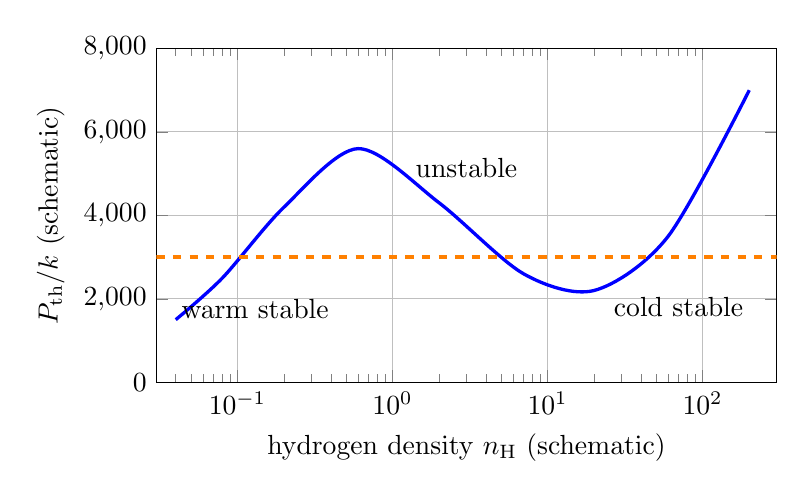
\begin{tikzpicture}
\begin{semilogxaxis}[
 width=0.78\linewidth,height=0.48\linewidth,
 xlabel={hydrogen density $n_{\rm H}$ (schematic)},
 ylabel={$P_{\rm th}/k$ (schematic)},
 xmin=0.03,xmax=300,ymin=0,ymax=8000,
 grid=major,
]
 \addplot[very thick,blue,smooth] coordinates {
 (0.04,1500) (0.08,2500) (0.2,4200) (0.6,5600)
 (2.0,4300) (7.0,2600) (20,2200) (60,3500) (200,7000)};
 \addplot[very thick,dashed,orange] coordinates {(0.03,3000) (300,3000)};
 \node at (axis cs:0.13,1750) {warm stable};
 \node at (axis cs:3.0,5150) {unstable};
 \node at (axis cs:70,1800) {cold stable};
\end{semilogxaxis}
\end{tikzpicture}
\caption{Original schematic of a two-phase thermal-equilibrium curve.  The shape is
pedagogical rather than a numerical cooling calculation.  A horizontal pressure can
intersect warm and cold stable branches, with an intermediate unstable solution.
Radiation field, metallicity, dust, cosmic rays, and shielding shift the curve.}
\label{fig:two-phase-schematic}
\end{figure}

\section{Working inventory of ISM regimes}

Table~\ref{tab:ism-regime-inventory} gives orientation values.  They are deliberately
shown as broad ranges; a phase label should never replace a measured density or
temperature.

\begin{table}[tbp]
\centering
\caption{Orientation map for interstellar regimes.  Values vary with galactic
environment and are not classification boundaries.}
\label{tab:ism-regime-inventory}
\begin{tabularx}{\textwidth}{@{}
 >{\raggedright\arraybackslash}p{0.18\textwidth}
 >{\raggedright\arraybackslash}p{0.15\textwidth}
 >{\raggedright\arraybackslash}p{0.16\textwidth}
 >{\raggedright\arraybackslash}X@{}}
\toprule
Regime & Typical $T$ & Indicative $n_{\rm H}$ & Representative probes \\
\midrule
Cold neutral medium & tens to a few hundred K &
$\sim1$--$10^2\,\mathrm{cm^{-3}}$ & H\,I 21-cm absorption/emission,
C\,I fine structure, [C\,II], Na\,I, K\,I \\
Warm neutral medium & several $10^3$--$10^4$ K &
$\sim0.1$--$1\,\mathrm{cm^{-3}}$ & H\,I 21 cm, UV low-ion absorption,
broad H\,I absorption \\
Warm ionized medium & roughly $10^4$ K &
$\sim10^{-2}$--$1\,\mathrm{cm^{-3}}$ & H$\alpha$, radio free--free,
pulsar dispersion, [N\,II], [S\,II] \\
Classical H\,II region & roughly $10^4$ K &
$\sim10$--$10^4\,\mathrm{cm^{-3}}$ & H and He recombination lines,
[O\,II], [O\,III], [N\,II], [S\,II] \\
Hot ionized medium & $10^5$--$10^7$ K &
$\sim10^{-4}$--$10^{-2}\,\mathrm{cm^{-3}}$ & soft X-ray lines and
continuum, O\,VI at interfaces, highly ionized absorption \\
Diffuse molecular gas & $\sim20$--$100$ K &
$\sim10^2$--$10^3\,\mathrm{cm^{-3}}$ & CO, CH, OH, HCO$^+$ absorption,
dust, gamma rays \\
Dense molecular structures & $\sim10$--$100$ K &
$\gtrsim10^4\,\mathrm{cm^{-3}}$ & NH$_3$, N$_2$H$^+$, HCN, HCO$^+$,
CS, dust continuum \\
\bottomrule
\end{tabularx}
\end{table}

The hot phase has large volume filling potential but small mass density; molecular
structures carry substantial mass in a small volume.  Filling factors are scale and
environment dependent.  A pencil-beam absorption spectrum samples column-weighted
material, while diffuse emission weights emissivity and telescope beam.  Apparent
disagreement can therefore reflect different selection functions rather than
inconsistent physics.

\subsection{Neutral atomic gas and the 21-cm line}

The H\,I hyperfine transition at 1420.4058~MHz connects the triplet and singlet
ground-state configurations.  Its excitation is described by a spin temperature
$T_s$.  For a homogeneous layer in the Rayleigh--Jeans limit,
\begin{equation}
 T_B(v)=T_{\rm bg}e^{-\tau(v)}+T_s\left[1-e^{-\tau(v)}\right].
 \label{eq:hi-transfer}
\end{equation}
Against a bright continuum source, absorption constrains $\tau(v)$; emission and
absorption together constrain $T_s$.  In the optically thin limit,
\begin{equation}
 N_{\rm HI}=1.823\times10^{18}
 \int T_B(v)\,\mathrm{d}v
 \quad\mathrm{cm^{-2}},
 \label{eq:hi-thin-column}
\end{equation}
with $T_B$ in kelvin and $v$ in $\mathrm{km\,s^{-1}}$.  Cold opaque components cause
the optically thin estimate to miss column.  Beam mismatch between emission and
pencil-beam absorption adds another systematic.

Thermal H\,I width sets an upper limit on temperature because turbulence also
broadens the profile.  Decomposing emission into Gaussians does not uniquely assign
physical clouds; regularization and component-count assumptions can dominate the
phase fractions.

\subsection{Warm ionized and hot gas}

Diffuse warm ionized gas is traced by recombination emission, free--free emission,
Faraday rotation, and pulsar dispersion measure
\begin{equation}
 {\rm DM}=\int n_e\,\mathrm{d}\ell.
 \label{eq:dispersion-measure}
\end{equation}
Combining DM with an emission measure $\int n_e^2\mathrm{d}\ell$ can constrain a
characteristic density and filling factor, provided the paths match.  Elevated
low-ionization line ratios in diffuse gas reflect its ionization and heating state and
can contaminate classifications based on integrated galaxy spectra.

Hot gas emits bremsstrahlung and metal lines in the extreme ultraviolet and X-ray.
Its inferred density depends on an emission measure and volume, hence on geometry and
filling factor.  Soft X-ray absorption by foreground gas complicates the coolest hot
components.  Intermediate-temperature ions at interfaces may be far from ionization
equilibrium, making single-temperature CIE fits an approximation.

\section{Photodissociation regions}

A photodissociation region (PDR) is predominantly neutral gas whose heating and
chemistry are controlled substantially by far-ultraviolet photons below the hydrogen
ionization edge.  PDRs occur on molecular-cloud surfaces, within clumpy clouds, around
H\,II regions, in diffuse atomic gas, and on galaxy-wide scales
\citep{HollenbachTielens1999}.  The term describes a regulatory regime, not a simple
geometric shell.

Two useful control parameters are gas density and incident far-UV field.  The latter
is often normalized as $G_0$ to a conventional interstellar band-integrated field, or
as $\chi$ under a different normalization.  These conventions differ; the unit and
reference field must be stated.  Ratios such as $G_0/n_{\rm H}$ influence grain
charging, photoelectric heating efficiency, and the location of chemical transitions.

\begin{figure}[tbp]
\centering
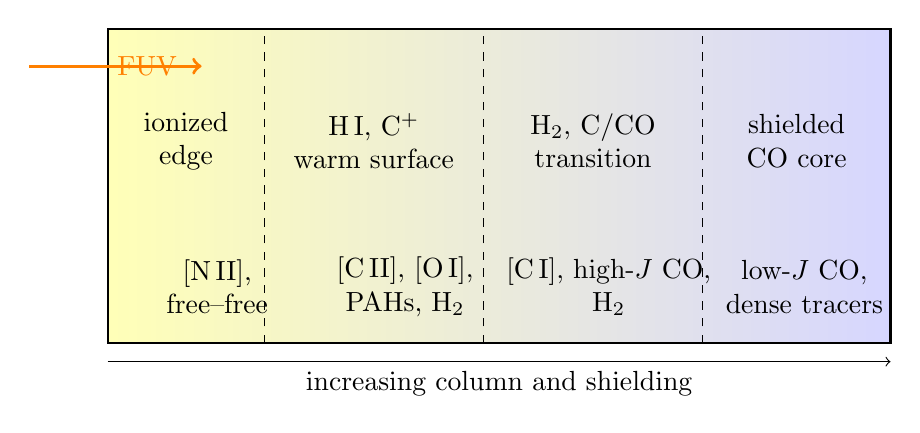
\begin{tikzpicture}[x=0.82\linewidth,y=0.95cm]
 \shade[left color=yellow!28,right color=blue!16] (0,0) rectangle (1,4.2);
 \draw[thick] (0,0) rectangle (1,4.2);
 \draw[->,very thick,orange] (-0.10,3.7)--(0.12,3.7)
   node[left=5pt] {FUV};
 \draw[dashed] (0.20,0)--(0.20,4.2);
 \draw[dashed] (0.48,0)--(0.48,4.2);
 \draw[dashed] (0.76,0)--(0.76,4.2);
 \node[align=center] at (0.10,2.7) {ionized\\edge};
 \node[align=center] at (0.34,2.7) {H\,I, C$^+$\\warm surface};
 \node[align=center] at (0.62,2.7) {H$_2$, C/CO\\transition};
 \node[align=center] at (0.88,2.7) {shielded\\CO core};
 \node[align=center] at (0.14,0.75) {[N\,II],\\free--free};
 \node[align=center] at (0.38,0.75) {[C\,II], [O\,I],\\PAHs, H$_2$};
 \node[align=center] at (0.64,0.75) {[C\,I], high-$J$ CO,\\H$_2$};
 \node[align=center] at (0.89,0.75) {low-$J$ CO,\\dense tracers};
 \draw[->] (0,-0.25)--(1,-0.25)
   node[midway,below] {increasing column and shielding};
\end{tikzpicture}
\caption{Original plane-parallel PDR concept.  Real clouds are porous and illuminated
from multiple directions, so zones overlap in projection.  Transition depths depend
on density, metallicity, dust, radiation spectrum, cosmic rays, and dynamics.}
\label{fig:pdr-layering}
\end{figure}

\subsection{Hydrogen formation and shielding}

In ordinary dusty gas, H$_2$ forms efficiently on grain surfaces.  A schematic
formation rate per volume is
\begin{equation}
 \mathcal{R}_{\rm form}=R_{\rm d}\,n_{\rm H}\,n({\rm H}),
 \label{eq:h2-formation}
\end{equation}
where $R_{\rm d}$ depends on grain abundance, temperature, and sticking physics.  The
unshielded photodissociation rate is reduced by dust attenuation and H$_2$
self-shielding:
\begin{equation}
 \mathcal{R}_{\rm diss}=D_0G_0\,
 f_{\rm sh}(N_{\rm H_2})e^{-\sigma_{d}N_{\rm H}}
 n({\rm H_2}).
 \label{eq:h2-dissociation}
\end{equation}
The H/H$_2$ transition occurs where formation balances the attenuated destruction.
H$_2$ can self-shield through its line spectrum at columns where CO remains
photodissociated.  This produces ``CO-faint'' or ``CO-dark'' molecular gas, especially
at low metallicity where dust shielding per hydrogen nucleus is smaller.

\subsection{Worked example: an \texorpdfstring{H$_2$}{H2} formation time}

Adopt $R_d=3\times10^{-17}\,\mathrm{cm^3\,s^{-1}}$ as an illustrative Milky-Way
value and $n_{\rm H}=100\,\mathrm{cm^{-3}}$.  The characteristic formation time from
mostly atomic gas is
\begin{equation}
 t_{\rm form}\sim(R_dn_{\rm H})^{-1}
 \simeq1.1\times10^7~\mathrm{yr}.
 \label{eq:h2-formation-time-example}
\end{equation}
At ten times higher density the time is roughly ten times shorter, absent changes in
grain properties.  Comparing this time with a turbulent crossing or cloud assembly
time tests chemical equilibrium.  The calculation does not locate the H/H$_2$
front, because photodissociation and shielding were omitted.

\subsection{Carbon chemistry and principal coolants}

At an illuminated surface, carbon is often C$^+$ while hydrogen may already be
neutral.  Increasing shielding permits neutral carbon and eventually CO to become
abundant.  This cartoon is chemically useful but not a strict series of planar
layers: turbulent mixing, cosmic rays, clumping, and nonequilibrium reactions can
place C$^+$, C, and CO together.

[C\,II] $158\,\mu$m and [O\,I] $63\,\mu$m are major coolants over portions of PDR
parameter space.  Their intensities relative to far-infrared dust emission and to one
another are commonly compared with PDR grids to infer density and radiation field.
Degeneracies are common, [C\,II] has ionized-gas contributions, [O\,I] can be optically
thick and self-absorbed, and multiple cloud faces occur within a beam.  A fitted
``$G_0$'' is therefore an effective model parameter unless geometry is constrained.

The photoelectric heating efficiency falls when grains become more positively
charged because electrons are harder to eject.  This helps explain why line-to-FIR
ratios can decline in intense radiation fields, but high gas density, dust-bounded
ionized regions, line opacity, and continuum optical depth can contribute to observed
``line deficits.''

\section{Molecular clouds are dynamical structures}

Molecular clouds are organized hierarchically into complexes, filaments, clumps,
cores, and velocity-coherent structures.  Boundaries defined by CO intensity,
extinction, or a dendrogram need not select the same mass.  A cloud catalog is the
output of a segmentation algorithm and resolution scale as well as an astrophysical
population.

For a structure of mass $M$, effective radius $R$, and one-dimensional velocity
dispersion $\sigma$, the commonly quoted virial parameter is
\begin{equation}
 \alpha_{\rm vir}=\frac{5\sigma^2R}{GM}
 \label{eq:virial-parameter}
\end{equation}
for an idealized uniform sphere without surface pressure or magnetic terms.  Values
near two are often associated with a marginally bound object under particular density
profiles.  Treating equation~\eqref{eq:virial-parameter} as an exact binding criterion
ignores geometry, density gradients, external pressure, magnetic support, mass
uncertainty, and time dependence \citep{McKeeOstriker2007}.

The turbulent Mach number is
\begin{equation}
 \mathcal{M}=\frac{\sigma_{\rm 3D}}{c_s},
 \qquad c_s=\sqrt{\frac{kT}{\mu m_{\rm H}}}.
 \label{eq:mach-number}
\end{equation}
Molecular gas is commonly supersonic on cloud scales.  Shocks create density
structure and dissipate energy; turbulence can both support a region globally and
compress subregions locally.  Line width includes opacity broadening, multiple
components, systematic gradients, and unresolved feedback in addition to turbulence.

\subsection{CO as a mass tracer}

For the CO $J=1\rightarrow0$ line,
\begin{equation}
 N({\rm H_2})=X_{\rm CO}W_{\rm CO},
 \qquad
 M_{\rm mol}=\alpha_{\rm CO}L'_{\rm CO}.
 \label{eq:xco-alpha-co}
\end{equation}
$X_{\rm CO}$ is a column conversion and $\alpha_{\rm CO}$ a luminosity-to-mass
conversion.  Authors must state whether helium is included.  CO(1--0) is usually
optically thick in individual clouds, yet integrated intensity can correlate with
mass because velocity structure exposes different surfaces and cloud-scale linewidth
and size correlate with mass.  This emergent calibration is environmental rather than
fundamental \citep{BolattoWolfireLeroy2013}.

At low metallicity, the H$_2$-bearing envelope outside the CO-rich region becomes a
larger fraction of the cloud, increasing $X_{\rm CO}$.  In warm, high-dispersion
galaxy centers or starbursts, CO luminosity per unit mass can rise, lowering
$\alpha_{\rm CO}$.  Dust-based gas masses offer an independent route but require
dust temperature, opacity, dust-to-gas ratio, and subtraction of atomic gas.

\subsection{Worked example: CO luminosity to molecular mass}

Let a galaxy have
$L'_{\rm CO(1-0)}=2.0\times10^9\,
\mathrm{K\,km\,s^{-1}\,pc^2}$.  Adopting
$\alpha_{\rm CO}=4.35\,
M_\odot(\mathrm{K\,km\,s^{-1}\,pc^2})^{-1}$ including helium gives
\begin{equation}
 M_{\rm mol}=8.7\times10^9\,M_\odot.
\end{equation}
If the environment instead justified
$\alpha_{\rm CO}=0.8$ in the same units, the mass would be
$1.6\times10^9\,M_\odot$.  The factor-of-five spread is a model uncertainty, not a
rounding error.  A publication should state the adopted conversion, environmental
rationale, transition ratio if a higher-$J$ line was observed, and helium convention.

\section{Dense-gas tracers and effective excitation}

Molecules with large dipole moments, such as HCN or HCO$^+$, have large spontaneous
rates and correspondingly high optically thin critical densities.  Calling one line
a ``dense-gas tracer'' does not mean it arises only above its tabulated critical
density.  Radiative trapping reduces effective critical density, multilevel cascades
alter populations, infrared pumping can matter, electron collisions can contribute,
and an extended density distribution emits over a broad range.

A more observationally relevant quantity is an effective excitation density: the
density required to produce a specified line brightness for an adopted column,
temperature, and radiation field.  It is model dependent by design.  Comparing
several transitions and isotopologues provides leverage on opacity and excitation.
Even then, abundance variations from freeze-out, photochemistry, shocks, or cosmic
rays may dominate ratios.

NH$_3$ inversion transitions provide a useful thermometer because ratios of
metastable states respond to kinetic temperature under common conditions.  N$_2$H$^+$
often survives where CO freezes onto grains, while CO desorption can destroy it.
SiO can be enhanced when shocks process grains.  These are chemical tendencies, not
one-to-one labels; the local reaction network and timescale determine the result.

\section{Dust, extinction, and continuum mass}

Optically thin thermal dust emission is commonly modeled as
\begin{equation}
 S_{\nu,\rm obs}=\frac{(1+z)\,\kappa_{\nu,\rm rest}
 M_dB_{\nu,\rm rest}(T_d)}{D_L^2},
 \label{eq:dust-mass-flux}
\end{equation}
under one widespread convention for opacity per dust mass.  Factors of $4\pi$ differ
among emissivity definitions, so dimensional consistency with the adopted $\kappa$
is essential.  A single modified blackbody compresses a temperature distribution
into an effective $T_d$; short-wavelength points weight warm dust and can bias mass
low.  At high optical depth, emission approaches $B_\nu(T)$ and no longer scales
linearly with mass.

Extinction measures a pencil-beam column weighted by grain cross section, whereas
emission measures dust luminosity and temperature.  Comparing them tests geometry and
opacity models.  Converting dust mass to total gas mass requires a dust-to-gas ratio
that varies with metallicity and chemical evolution.

\section{Shocks, interfaces, and phase exchange}

A shock converts bulk kinetic energy into heat, compression, magnetic energy, cosmic
rays, and radiation.  For a strong adiabatic shock in a monatomic gas, the immediate
post-shock temperature is approximately
\begin{equation}
 T_s=\frac{3\mu m_{\rm H}}{16k}v_s^2
 \simeq1.4\times10^5\,\mathrm{K}
 \left(\frac{\mu}{0.61}\right)
 \left(\frac{v_s}{100\,\mathrm{km\,s^{-1}}}\right)^2.
 \label{eq:shock-temperature}
\end{equation}
Radiative shocks develop a cooling and recombination zone that emits ions spanning a
large temperature range.  Their line ratios depend on shock speed, preshock density,
magnetic parameter, abundance, precursor radiation, and completeness of the cooling
zone \citep{DopitaSutherland2003}.

Conductive boundaries, turbulent mixing layers, and cloud ablation also populate
intermediate ions.  A sightline through many interfaces can produce substantial
columns without a large volume of gas at the ion's CIE peak temperature.  Kinematic
alignment, multiple ions, and cooling-time arguments are needed to distinguish
interfaces from a volume-filling phase.

\section{Combining tracers without forcing them into one phase}

A robust multiphase analysis uses a generative mixture rather than assigning each
line to exactly one component.  For line $\ell$,
\begin{equation}
 F_\ell=\sum_p F_{\ell,p}(T_p,n_p,Z_p,U_p,N_p,\ldots),
 \label{eq:multiphase-flux-sum}
\end{equation}
where phases $p$ may include ionized gas, atomic PDR surfaces, CO-faint H$_2$, and
shielded molecular gas.  The data constrain only combinations for which sufficiently
distinct tracers exist.  Priors on pressure balance, abundance continuity, or geometry
should be explicit and tested rather than assumed silently.

The following cross-checks are especially valuable:
\begin{itemize}
 \item compare H\,I emission with absorption to test opacity and spin temperature;
 \item use [N\,II] or other ionized-only lines to estimate the ionized contribution
 to [C\,II];
 \item compare CO-based gas with dust-based gas to expose CO-faint material or
 conversion-factor changes;
 \item use isotopologues and multiple $J$ levels to test CO opacity and excitation;
 \item compare density-squared emission with density-linear absorption or dispersion
 measures to constrain clumping;
 \item align velocity components before combining ionic ratios across transitions.
\end{itemize}
The ISM's complexity is not a failure of the phase framework.  It is the central
observable: line combinations map how matter cycles among thermal, chemical, and
dynamical states.
